% Тип документа
\documentclass[a4paper,12pt]{extarticle}

% Шрифты, кодировки, символьные таблицы, переносы
\usepackage{cmap}
\usepackage[T2A]{fontenc}
\usepackage[utf8x]{inputenc}
\usepackage[russian]{babel}

% Это пакет -- хитрый пакет, он нужен но не нужен
\usepackage[mode=buildnew]{standalone}

\usepackage
	{
		% Дополнения Американского математического общества (AMS)
		amssymb,
		amsfonts,
		amsmath,
		amsthm,
		physics,
		% misccorr,
		% 
		% Графики и рисунки
		wrapfig,
		graphicx,
		subcaption,
		float,
		tikz,
		tikz-3dplot,
		caption,
		csvsimple,
		color,
		booktabs,
		pgfplots,
		pgfplotstable,
		geometry,
		% 
		% Таблицы, списки
		makecell,
		multirow,
		indentfirst,
		%
		% Интегралы и прочие обозначения
		ulem,
		esint,
		esdiff,
		% 
		% Колонтитулы
		fancyhdr,
	}  

\usepackage{xcolor}
\usepackage{hyperref}

 % Цвета для гиперссылок
\definecolor{linkcolor}{HTML}{000000} % цвет ссылок
\definecolor{urlcolor}{HTML}{799B03} % цвет гиперссылок
 
\hypersetup{pdfstartview=FitH,  linkcolor=linkcolor,urlcolor=urlcolor, colorlinks=true}
% Обводка текста в TikZ
\usepackage[outline]{contour}

% Увеличенный межстрочный интервал, французские пробелы
\linespread{1.3} 
\frenchspacing 

 
\usetikzlibrary
	{
		decorations.pathreplacing,
		decorations.pathmorphing,
		patterns,
		calc,
		scopes,
		arrows,
		fadings,
		through,
		shapes.misc,
		arrows.meta,
		3d,
		quotes,
		angles,
		babel
	}


\tikzset{
	force/.style=	{
		>=latex,
		draw=blue,
		fill=blue,
				 	}, 
	%				 	
	axis/.style=	{
		densely dashed,
		blue,
		line width=1pt,
		font=\small,
					},
	%
	th/.style=	{
		line width=1pt},
	%
	acceleration/.style={
		>=open triangle 60,
		draw=magenta,
		fill=magenta,
					},
	%
	inforce/.style=	{
		force,
		double equal sign distance=2pt,
					},
	%
	interface/.style={
		pattern = north east lines, 
		draw    = none, 
		pattern color=gray!60,
					},
	cross/.style=	{
		cross out, 
		draw=black, 
		minimum size=2*(#1-\pgflinewidth), 
		inner sep=0pt, outer sep=0pt,
					},
	%
	cargo/.style=	{
		rectangle, 
		fill=black!70, 
		inner sep=2.5mm,
					},
	%
	caption/.style= {
		midway,
		fill=white!20, 
		opacity=0.9
					},
	%
	}

\newenvironment{tikzpict}
    {
	    \begin{figure}[htbp]
		\centering
		\begin{tikzpicture}
    }
    { 
		\end{tikzpicture}
		% \caption{caption}
		% \label{fig:label}
		\end{figure}
    }


\newcommand{\vbLabel}[3]{\draw ($(#1,#2)+(0,5pt)$) -- ($(#1,#2)-(0,5pt)$) node[below]{#3}}
\newcommand{\vaLabel}[3]{\draw ($(#1,#2)+(0,5pt)$) node[above]{#3} -- ($(#1,#2)-(0,5pt)$) }

\newcommand{\hrLabel}[3]{\draw ($(#1,#2)+(5pt,0)$) -- ($(#1,#2)-(5pt,0)$) node[right, xshift=1em]{#3}}
\newcommand{\hlLabel}[3]{\draw ($(#1,#2)+(5pt,0)$) node[left, xshift=-1em]{#3} -- ($(#1,#2)-(5pt,0)$) }



\newcommand\zi{^{\,*}_i}
\newcommand\sumn{\sum_{i=1}^{N}}

\tikzset{
	coordsys/.style={scale=1.8,x={(1.1cm,-0cm)},y={(0.5cm,1cm)}, z={(0cm,0.8cm)}},
	coordsys/.style={scale=1.5,x={(0cm,0cm)},y={(1cm,0cm)}, z={(0cm,1cm)}}, 
	coordsys/.style={scale=1.5,x={(1cm,0cm)},y={(0cm,1cm)}, z={(0cm,0cm)}}, 
}

\usepgfplotslibrary{units}


% Draw line annotation
% Input:
%   #1 Line offset (optional)
%   #2 Line angle
%   #3 Line length
%   #5 Line label
% Example:
%   \lineann[1]{30}{2}{$L_1$}

\newcommand{\lineann}[4][0.5]{%
    \begin{scope}[rotate=#2, blue,inner sep=2pt, ]
        \draw[dashed, blue!40] (0,0) -- +(0,#1)
            node [coordinate, near end] (a) {};
        \draw[dashed, blue!40] (#3,0) -- +(0,#1)
            node [coordinate, near end] (b) {};
        \draw[|<->|] (a) -- node[fill=white, scale=0.8] {#4} (b);
    \end{scope}
}

\newcommand{\lineannn}[4][0.5]{%
    \begin{scope}[rotate=#2, blue,inner sep=2pt, ]
        \draw[dashed, blue!40] (0,0) -- +(0,#1)
            node [coordinate, near end] (a) {};
        \draw[dashed, blue!40] (#3,0) -- +(0,#1)
            node [coordinate, near end] (b) {};
        % \draw[color=white, color=blue] (a) -- node[fill=white, scale=0.8] {#4} (b);
        \draw[->|] (a)++(-0.3,0) -- (a);
        \draw[->|] (b)++(0.3,0) coordinate (xx) -- (b);
        \draw (xx) node[fill=white, scale=0.8, right] {#4};
    \end{scope}
}

% Круговая стрелка относительно центра (дуга из центра)
\tikzset{
  pics/carc/.style args={#1:#2:#3}{
    code={
      \draw[pic actions] (#1:#3) arc(#1:#2:#3);
    }
  },
  dash/.style={
  	dash pattern=on 5mm off 5mm
  }
}

% Среднее <#1>
\newcommand{\mean}[1]{\langle#1\rangle}

\pgfplotsset{
    % most recent feature set of pgfplots
    compat=newest,
}

% const прямым шрифтом
\newcommand\ct[1]{\text{\rmfamily\upshape #1}}
\newcommand*{\const}{\ct{const}}


\usepackage[europeanresistors,americaninductors]{circuitikz}

% Style to select only points from #1 to #2 (inclusive)
\pgfplotsset{select/.style 2 args={
    x filter/.code={
        \ifnum\coordindex<#1\def\pgfmathresult{}\fi
        \ifnum\coordindex>#2\def\pgfmathresult{}\fi
    }
}}


\usepackage{array}
\usepackage{pstool}


%%%%%%%%%%%%%%%%%%%%%%%%%%%%%%%%%%%%%%%%%%%%%%%%%
\makeatletter
\newif\if@gather@prefix 
\preto\place@tag@gather{% 
  \if@gather@prefix\iftagsleft@ 
    \kern-\gdisplaywidth@ 
    \rlap{\gather@prefix}% 
    \kern\gdisplaywidth@ 
  \fi\fi 
} 
\appto\place@tag@gather{% 
  \if@gather@prefix\iftagsleft@\else 
    \kern-\displaywidth 
    \rlap{\gather@prefix}% 
    \kern\displaywidth 
  \fi\fi 
  \global\@gather@prefixfalse 
} 
\preto\place@tag{% 
  \if@gather@prefix\iftagsleft@ 
    \kern-\gdisplaywidth@ 
    \rlap{\gather@prefix}% 
    \kern\displaywidth@ 
  \fi\fi 
} 
\appto\place@tag{% 
  \if@gather@prefix\iftagsleft@\else 
    \kern-\displaywidth 
    \rlap{\gather@prefix}% 
    \kern\displaywidth 
  \fi\fi 
  \global\@gather@prefixfalse 
} 
\newcommand*{\beforetext}[1]{% 
  \ifmeasuring@\else
  \gdef\gather@prefix{#1}% 
  \global\@gather@prefixtrue 
  \fi
} 
\makeatother
%%%%%%%%%%%%%%%%%%%%%%%%%%%%%%%%%%%%%%%%%%%%%%%%%

\geometry		
	{
		left			=	2cm,
		right 			=	2cm,
		top 			=	3cm,
		bottom 			=	3cm,
		bindingoffset	=	0cm
	}

%%%%%%%%%%%%%%%%%%%%%%%%%%%%%%%%%%%%%%%%%%%%%%%%%%%%%%%%%%%%%%%%%%%%%%%%%%%%%%%



	%применим колонтитул к стилю страницы
\pagestyle{fancy} 
	%очистим "шапку" страницы
\fancyhead{} 
	%слева сверху на четных и справа на нечетных
\fancyhead[R]{\labauthors} 
	%справа сверху на четных и слева на нечетных
\fancyhead[L]{Отчёт по лабораторной работе №\labnumber} 
	%очистим "подвал" страницы
\fancyfoot{} 
	% номер страницы в нижнем колинтуле в центре
\fancyfoot[C]{\thepage} 

%%%%%%%%%%%%%%%%%%%%%%%%%%%%%%%%%%%%%%%%%%%%%%%%%%%%%%%%%%%%%%%%%%%%%%%%%%%%%%%

\renewcommand{\contentsname}{Оглавление}

\usepackage{tocloft}
% \renewcommand{\cftpartleader}{\cftdotfill{\cftdotsep}} % for parts
% \renewcommand{\cftsectiondotsep}{\cftdotsep}% Chapters should use dots in ToC
\renewcommand{\cftsecleader}{\cftdotfill{\cftdotsep}}
%\renewcommand{\cftsecleader}{\cftdotfill{\cftdotsep}} % for sections, if you really want! (It is default in report and book class (So you may not need it).
% ---------
% \newcommand{\cftchapaftersnum}{.}%
% \usepackage{titlesec}
% \titlelabel{\thetitle.\quad}
\usepackage{secdot}
\sectiondot{subsection}

\begin{document}

\def\labauthors{Сарафанов Ф.Г., Понур К.А., Сидоров Д.А.}
\def\labgroup{430}
\def\labnumber{1}
\def\labtheme{Исследование фотоэффекта и измерение постоянной Планка}
\renewcommand{\vec}{\mathbf}
\renewcommand{\Re}{\operatorname{Re}}
\renewcommand{\Im}{\operatorname{Im}}
\renewcommand{\phi}{\varphi}
\renewcommand{\hat}{\widehat}

\begin{titlepage}

\begin{center}

{\small\textsc{Нижегородский государственный университет имени Н.\,И. Лобачевского}}
\vskip 1pt \hrule \vskip 3pt
{\small\textsc{Радиофизический факультет}}

\vfill

{\Large Отчет по лабораторной работе №\labnumber\vskip 12pt\bfseries \labtheme}
	
\end{center}

\vfill
	
\begin{flushright}
	{Выполнили студенты \labgroup\ группы\\ \labauthors}%\vskip 12pt Принял:\\ Менсов С.\,Н.}
\end{flushright}
	
\vfill
	
\begin{center}
	Нижний Новгород, \the\year
\end{center}

\end{titlepage}



\tableofcontents
\newpage

\section{Теоретическая часть}
\subsection*{Фотоэффект}
В настоящее время в науке, технике и быту широкое приме¬нение получили фотоэлементы - электровакуумные или полу¬проводниковые приборы, преобразующие энергию электромагнитного излучения оптического диапазона в электрическую. Действие этих приборов основано на использовании фотоэлектрических эффектов (фотоэффектов). 
Существует два вида фотоэффекта: внешний и внутренний. Внешний фотоэффект (фотоэлектронная эмиссия) заключается в испускании поверхностью тела электронов во внешнее пространство (вакуум или газ) под действием падающей на эту поверхность световой энергии. Внутренним фотоэффектом называется изменение под действием световой энергии проводимости тел вследствие появления добавочных электронов проводимости, либо эффект разделения зарядов в облу¬чаемом светом теле, что приводит к возникновению электродвижущей силы (фотогальванический эффект). Внешний фотоэффект используется в вакуумных и газонаполненных фотоэлементах, а также в фотоумножителях; внутренний - в полупроводниковых фотоэлементах: фото резисторах, фотодиодах и фототранзисторах (в том числе, в солнечных батареях).
В данной работе исследуется внешний фотоэффект. При этом используется вакуумный фотоэлемент, имеющий два электрода - катод, эмитирующий электроны под действием света, и анод - коллектор электронов. Если на анод подать положительный потенциал, то во внешней цепи прибора потечет ток, называемый фототоком. Величина фототока зависит от интенсивности света и материала катода. При увеличении потенциала анода фототок сначала увеличивается, а затем достигает насыщения (все электроны, испускаемые катодом, достигают анода, и при дальнейшем увеличении анодного напряжения величина тока не меняется).
Основные законы внешнего фотоэффекта, установленные экспериментально, состоят в следующем.
\begin{enumerate}
 	\item Величина фототока в режиме насыщения при неизменном спектральном составе излучения прямо пропорциональна интенсивности падающего света (закон Столетова).
	 \item Для каждого вещества существует длинноволновая граница фотоэффекта $\lambda_0$, за которой (при $\lambda>\lambda_0$) фотоэмиссия не наблюдается.
	 \item Максимальная кинетическая энергия электронов $W_{max}$ при фотоэффекте линейно возрастает с увеличением частоты падающего света $\nu$ и не зависит от его интенсивности: $W\propto \nu$.
\end{enumerate}

Эти законы просто объясняются на основании квантовой теории света и электронной теории твердого тела. Согласно квантовой теории, свет имеет дуальную природу: он обладает не только волновыми свойствами, но и свойствами частиц и может быть представлен в виде потока квантов света (фотонов). Энергия одного фотона пропорциональна частоте соответствующей волны: $E=h \nu$, где $h$-- постоянная Планка, по современным данным равная $6.6260755(40)\cdot10^{-34}$ Дж$\cdot$с

Излучение света на элементарном уровне идет отдельными квантами. Рассмотрим процесс фотоэмиссии из металла Поскольку каждый фотон действует на электроны твердого тела независимо от других фотонов, причем существует определенная вероятность $Р$ того, что это действие приведет к эмиссии электрона, то при попадании на катод $N$ фотонов в секунду электронный ток с него составит $n=NP$ электронов в секунду. Интенсивность падающего на фотокатод света согласно квантовой теории также пропорциональна $N: I\propto Nhv$. Таким образом образом объясняется закон Столетова.

\begin{figure}[h]
	\centering
	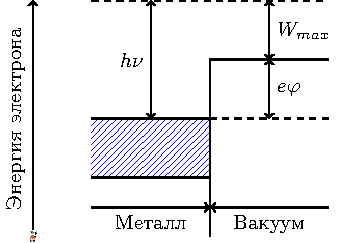
\includegraphics[]{fig/fig1}
	\caption{}
	\label{fig:1}
\end{figure}
Согласно электронной теории твердого тела, электроны проводимости в металле находятся в потенциальной яме и при достаточно низкой температуре равномерно распределены по энергиям, заполняя потенциальную яму до некоторого уровня (см. рис. \ref{fig:1}).
Наименьшая энергия, необходимая электрону для выхода в вакуум, называется работой выхода: $U_{\text{вых}} = e\phi$, где $е$ - заряд электрона. То же название обычно употребляют и для потенциала $\phi$, так как энергию в атомной физике принято измерять в электрон-вольтах. Максимальная энергия, которую может получить электрон при соударении с фотоном, равна $h \nu$. Очевидно, при $h \nu<e\phi$ фотоэмиссия невозможна, что объясняет существование красной границы.

Из рис.\ref{fig:1} также следует, что максимальная кинетическая энергия электрона равна
\begin{equation}
	\label{eq:1}
 	W_{max}=h \nu -e\phi
 \end{equation} 

Это уравнение (уравнение Эйнштейна) объясняет третий закон
фотоэффекта. Электроны, выбиваемые с более глубоких энергетических уровней, имеют меньшую кинетическую энергию.

Максимальную кинетическую энергию электронов $W_{max}K$ можно определить, если между анодом и катодом фотоэлемента создать тормозящее электроны поле. Для этого на анод подается отрицательный по отношению к катоду потенциал $V$. Вылетевшие из фотокатода электроны имеют различные энергии. Те электроны, энергия которых удовлетворяет условию $W < e\cdot V$, не могут достичь анода. Поэтому при увеличении $ |V|$ фототок уменьшается. При некотором значении $V = V_{3}$ (потенциал запирания) даже наиболее быстрые электроны не смогут достичь анода, и ток прекратится. При этом
\begin{equation}
	\label{eq:2}
	W_{max}=e\cdot V_{3}
\end{equation}
Из уравнений (\ref{eq:1}) и (\ref{eq:2}) найдём линейное соотношение между потенциалом запирания и частотой падающего света
\begin{equation}
	\label{eq:3}
	V_{3}=\frac h\nu \nu-\phi
\end{equation}

Экспериментальная проверка формулы Эйнштейна была впервые осуществлена Ричардсоном и Комптоном в 1912 г., более тщательно - Милликеном в 1916 г. Обе работы подтвердили формулу (\ref{eq:3}). Наиболее точная проверка была проведена Лукирским и Прилежаевым в 1926г.

\section{Практическая часть}
\subsection{Описание эксперимента}
\begin{figure}[h!]
	\centering
	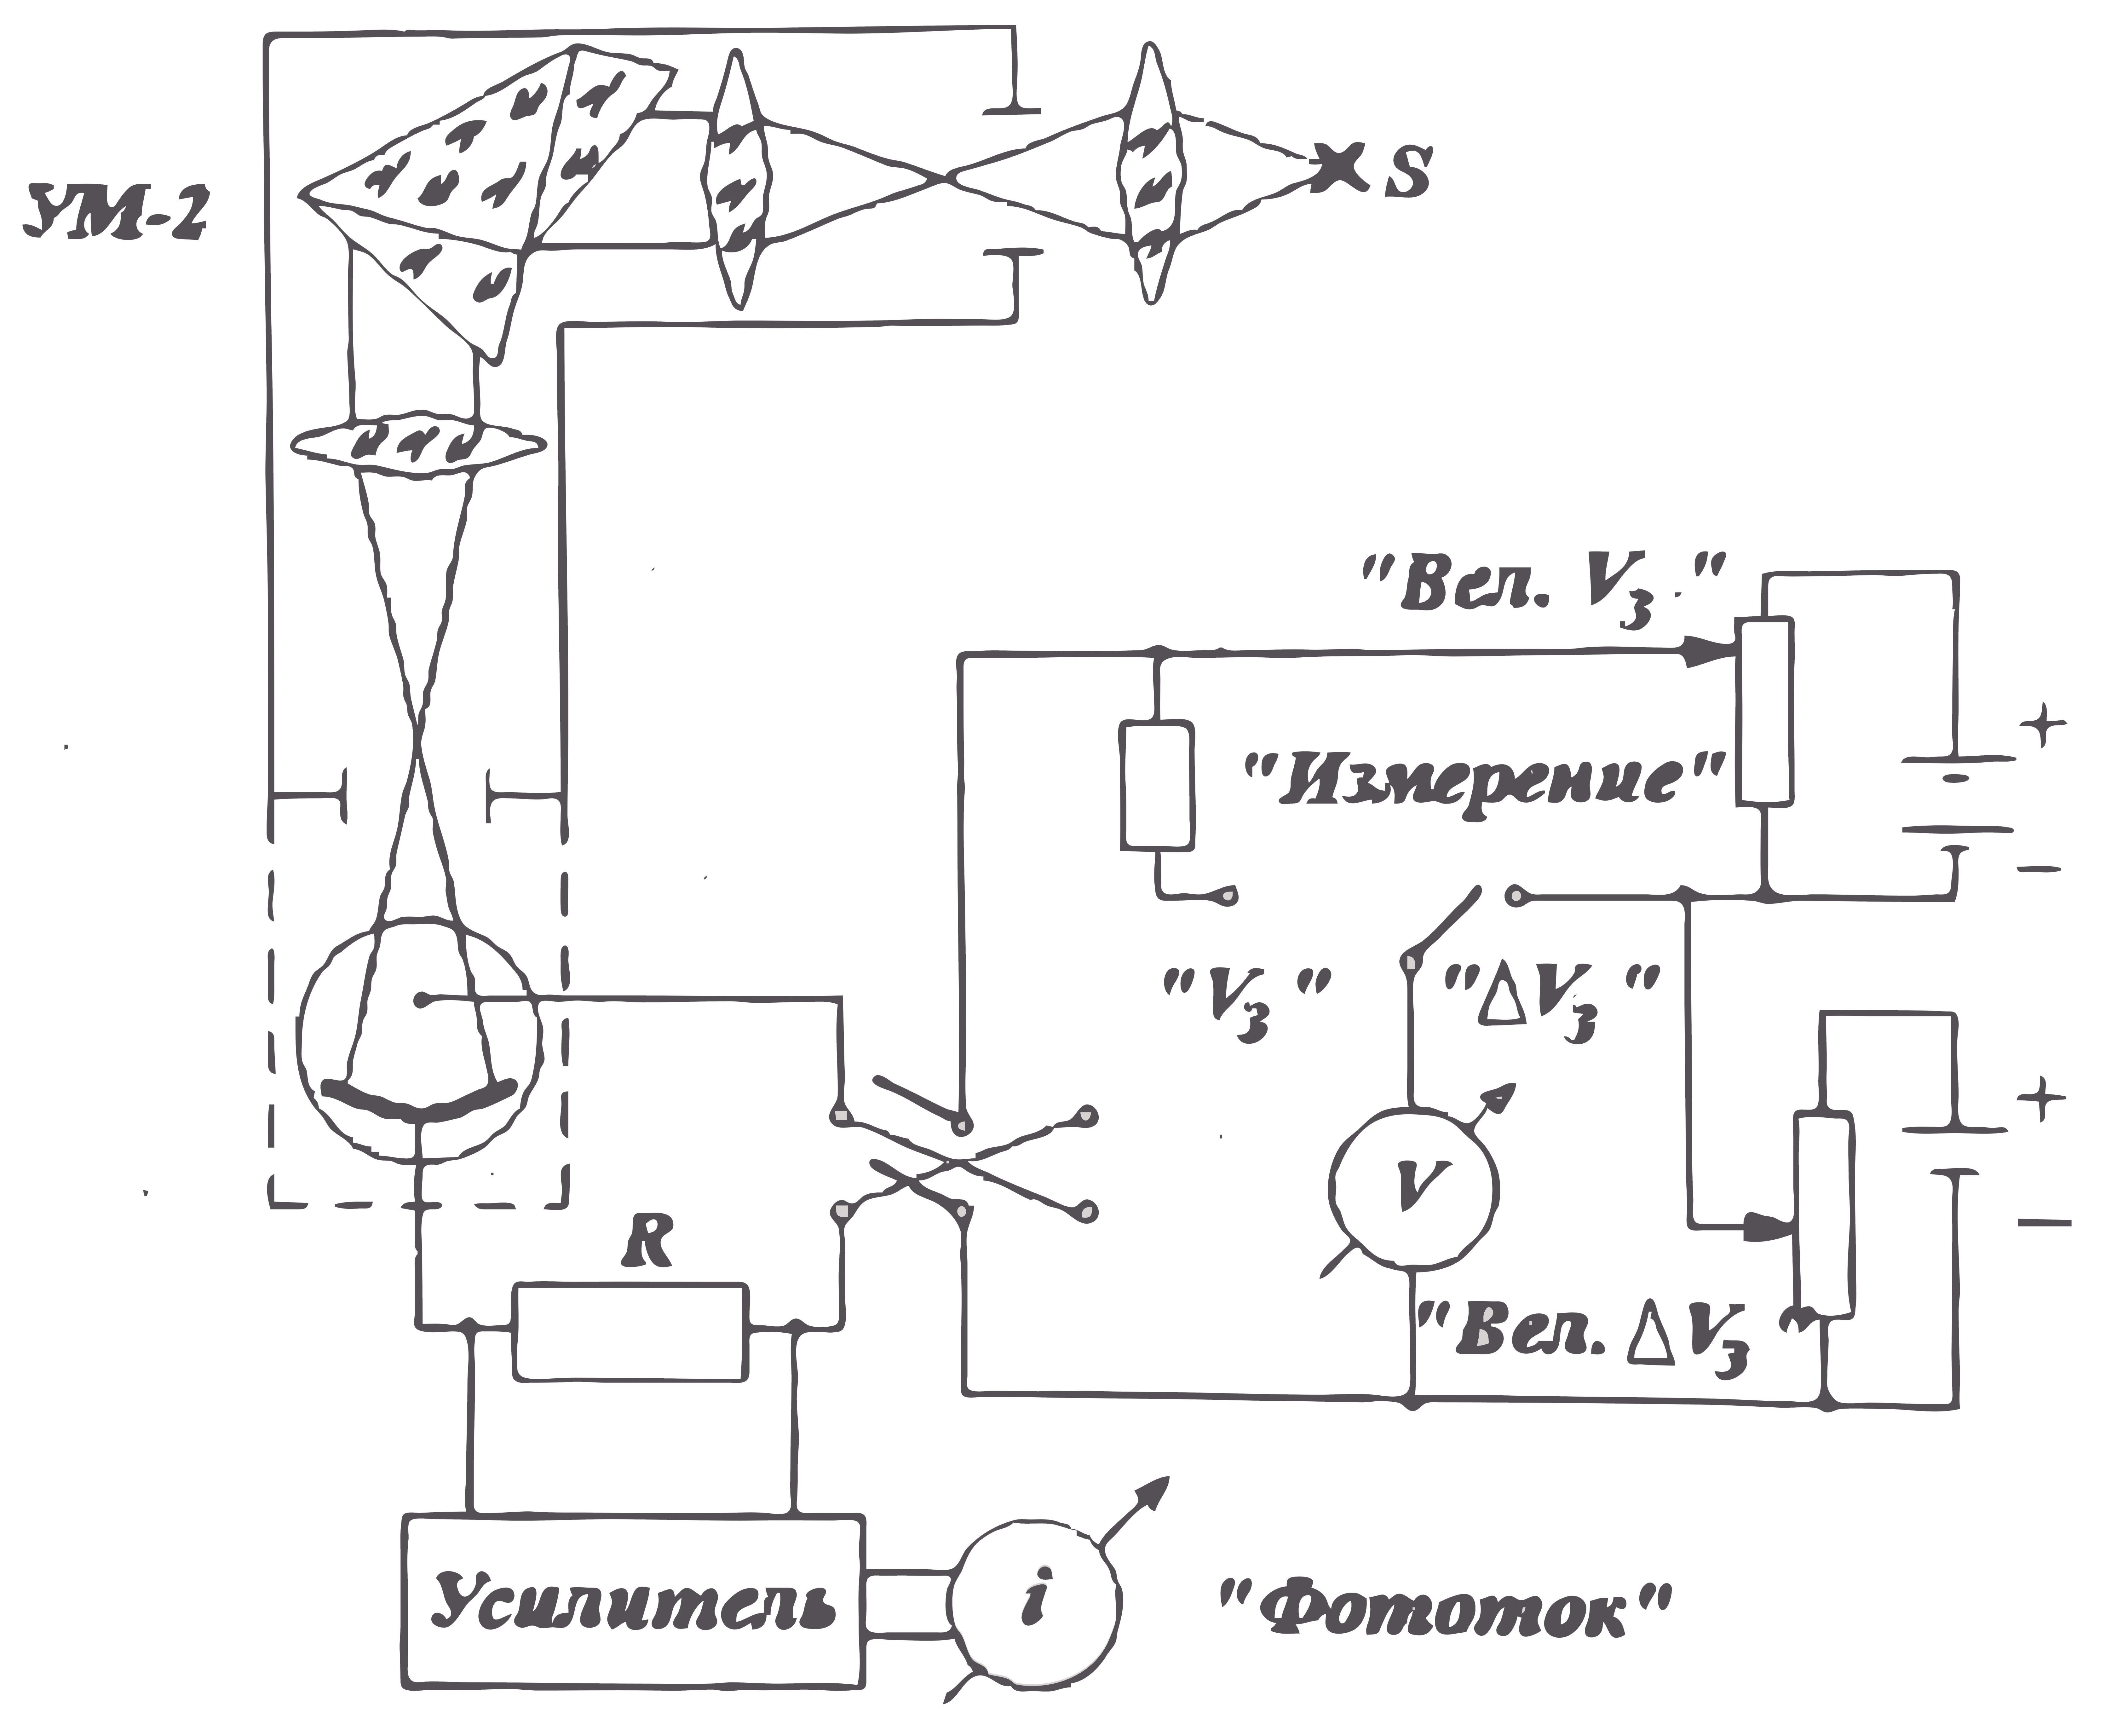
\includegraphics[width=\linewidth]{fig/fig2.png}
	\caption{Схема экспериментальной установки}
	\label{fig:2}
\end{figure}

Целью работы является проверка законов фотоэффекту а также измерение фундаментальной константы - постоянной Планка - на основании соотношения (\ref{eq:3}) между потенциалом запирания $V_{3}$ и частотой света $\nu$.

Схема установки приведена на рис. \ref{fig:2}. Свет от лампы накаливания или ртутной лампы фокусируется конденсором на входную щель призменного монохроматора УМ-2. В монохроматоре свет через входную щель, регулирующую световой потом, падает на объектив коллиматора и параллельным пучком проходит диспергирующую призму. Ввиду того, что фокусное расстояние объектива для каждой длины волны изменяется, предусмотрена возможность фокусировки объектива коллиматора. Фокусировочное движение осуществляется маховичком и контролируется по миллиметровой шкале с нониусом. В трубе коллиматора между щелью и объективом помещен затвор, с помощью которого можно прекратить доступ света в прибор. Под углом $90^{\circ}$ к падающему пучку света располагается выходная труба монохроматора. Поворачивая призменный столик на различные углы относительно падающего пучка света, получают свет различной длины волны, распространяющийся параллельно оси выходной трубы. Фокусируя свет в выходную плоскость, выделяют с помощью выходной щели узкий спектральный интервал. Прямо на выходной щели крепится фотоэлемент типа Ф-5, помещенный в металлический экран, предохраняющий от попадания паразитного света и от электрических наводок. Таким образом, поворачивая призму монохроматора, можно изменять частоту освещающего фотоэлемент света. На измерительном барабане поворотного механизма нанесены относительные деления-градусы поворота барабана. Отсчет читается против индекса, скользящего по спиральной канавке. Частота (длина волны) определяется по отсчету барабана монохроматора и градуировочному графику. Для градуировки прибора служит ртутная лампа.

Потенциал анода фотоэлемента можно менять с помощью двух потенциометров "Вел. V" и "Вел. $\Delta V$". Величина потенциала измеряется вольтметром при положении переключателя "Измерение" на "V" (шкала вольтметра при этом соответствует 2.5 В). В положении переключателя "$\Delta V$" измеряется лишь часть анодного напряжения, подаваемая с потенциометра "Вел. $\Delta V$" (шкала вольтметра на 0.25 В). Имеется переключатель знака анодного напряжения.

Возникающий в фотоэлементе ток при отрицательном потенциале анода (режим задержки) очень мал (порядка $10^{-11}$ А) и не может быть измерен непосредственно. Для его измерения служит балансный электрометрический усилитель. На вход усилителя подается напряжение, пропорциональное величине фототока, которое образуется на большом (порядка $10^9$ Ом) сопротивлении $R$, включенном в цепь фотоэлемента. Поэтому показания микроамперметра на выходе усилителя пропорциональны величине фототока.

Потенциал запирания определяется величиной тормозящего электроны анодного напряжения в момент исчезновения фототока. Следует подчеркнуть, что измеренное $V_{3}$ отличается от истинного значения
\begin{equation}
	V_0=V_{3}+C
\end{equation}
Величина поправки C зависит от ряда факторов, важнейшим из которых являются наличие обратного тока, вызванного вторичной электронной эмиссией с анода, и контактная разность потенциалов между анодом и катодом. Это приводит к большой погрешности 
при определении постоянной Планка по зависимости $V_{3}$ от $\nu$.

С целью увеличения точности опыта можно провести измерения для двух близких значений частоты света $\nu_1$ и $\nu_2$. Если частоты достаточно близки, то поправка $C$ практически не изменится (все остальные условия опыта останутся без изменения). Тогда разность $\Delta V_{3} = V_{3}(\nu_2)- V_{3}(\nu_1)$ будет совпадать с разностью истинных потенциалов запирания и, согласно уравнению (\ref{eq:3}), для определения постоянной Планка можно воспользоваться соотношением
\begin{equation}
	\Delta V_{3}=\frac he \Delta \nu,
\end{equation}
где $\Delta \nu= \nu_2- \nu_1$.

В этом методе необходимо достаточно точно знать значения частот $\nu_1$ и $\nu_2$. Точность определения частот по градуировочному графику монохроматора в случае применения источника белого света (лампа накаливания) невелика, поэтому необходимо использовать источник с линейчатым спектром, для которого частоты излучения измерены с высокой точностью. В данной работе применена ртутная лампа ДРШ-250. 

\subsection{Эксперимент}
Для того, чтобы установить связь между шкалой монохроматора УМ-2 будем пользоваться рис. \ref{fig:8}. 
\begin{figure}[H]
	\centering
	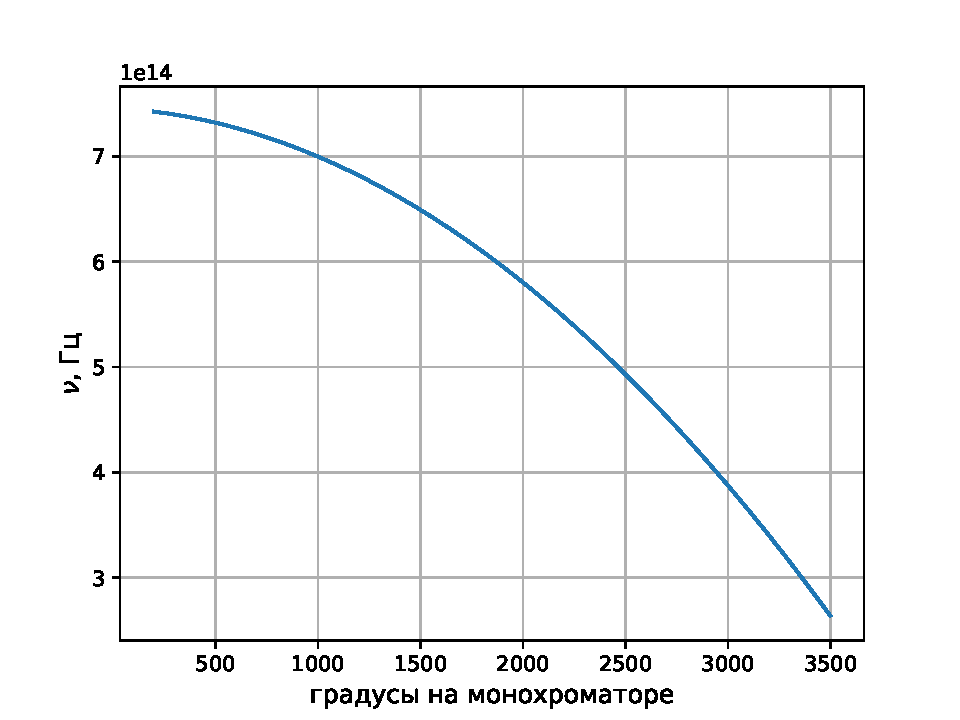
\includegraphics[scale=1]{scripts/podgon.pdf}
	\caption{}
	\label{fig:8}
\end{figure}

\section{Задание 1}
\begin{center}
    \begin{figure}[H]
        \begin{minipage}{0.49\linewidth}
            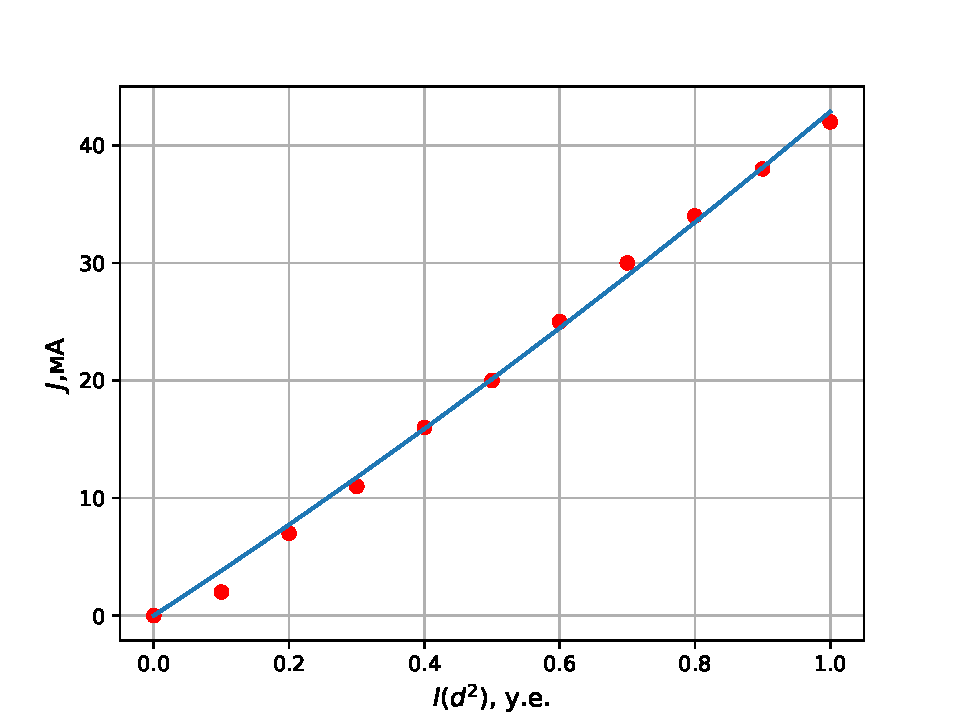
\includegraphics[width=\linewidth]{scripts/1500} 
            \vspace{-30pt}
            \label{fig:3}
            \captionof{subfigure}{} 
        \end{minipage}
    \begin{minipage}{0.49\linewidth}
        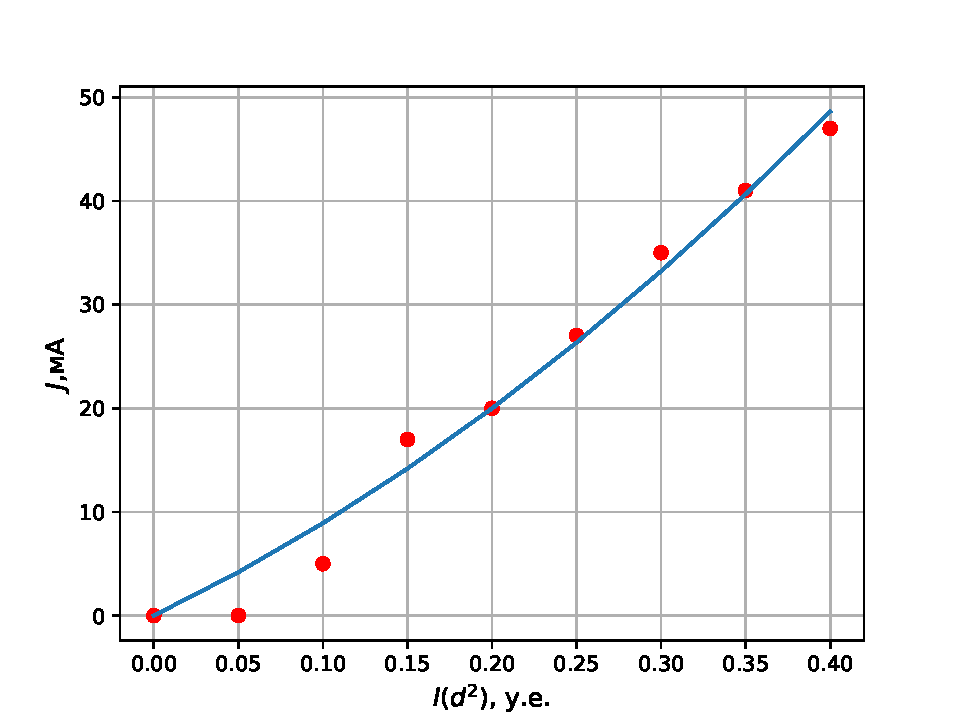
\includegraphics[width=\linewidth]{scripts/2000} 
        \vspace{-30pt}
        \label{fig:4}
        \captionof{subfigure}{} 
    \end{minipage}
    \end{figure}
\end{center}
\begin{center}
    \begin{figure}[H]

            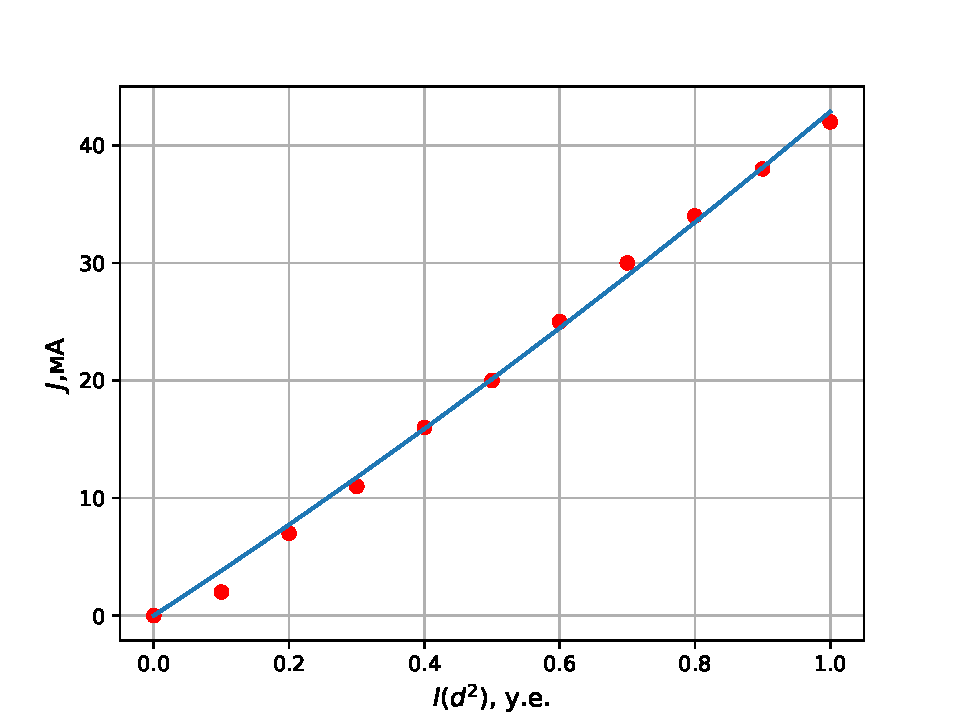
\includegraphics[scale=0.6]{scripts/1500} 
            \vspace{-30pt}
            \label{fig:3}
            \captionof{subfigure}{} 

    \end{figure}
\end{center}
% \begin{figure}[H]
% 	\centering
% 	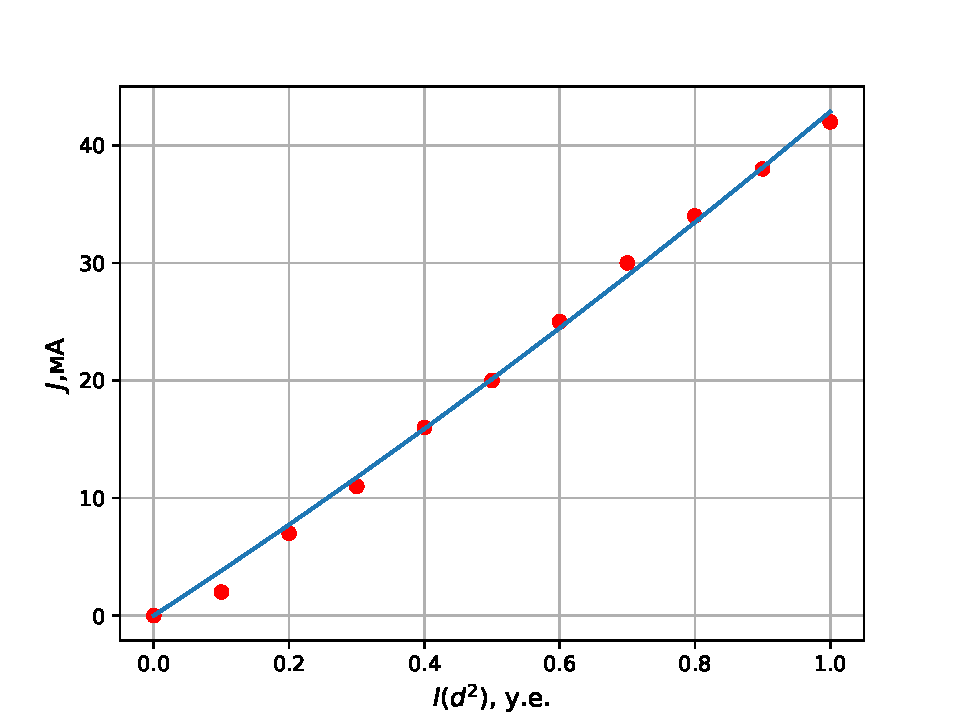
\includegraphics[scale=0.8]{scripts/1500}
% 	\caption{$1500^{\circ}$}{}
% 	\label{fig:3}

% \end{figure}
% \begin{figure}[H]
% 	\centering
% 	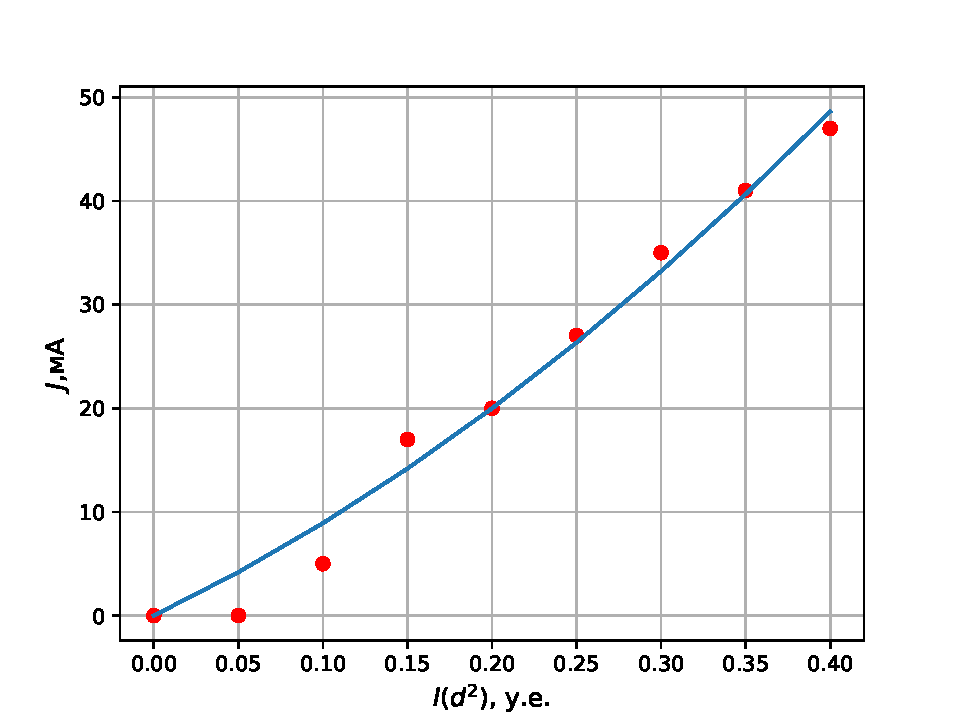
\includegraphics[scale=0.8]{scripts/2000}
% 	\caption{$2000^{\circ}$}
% 	\label{fig:4}
% \end{figure}
% \begin{figure}[H]
% 	\centering
% 	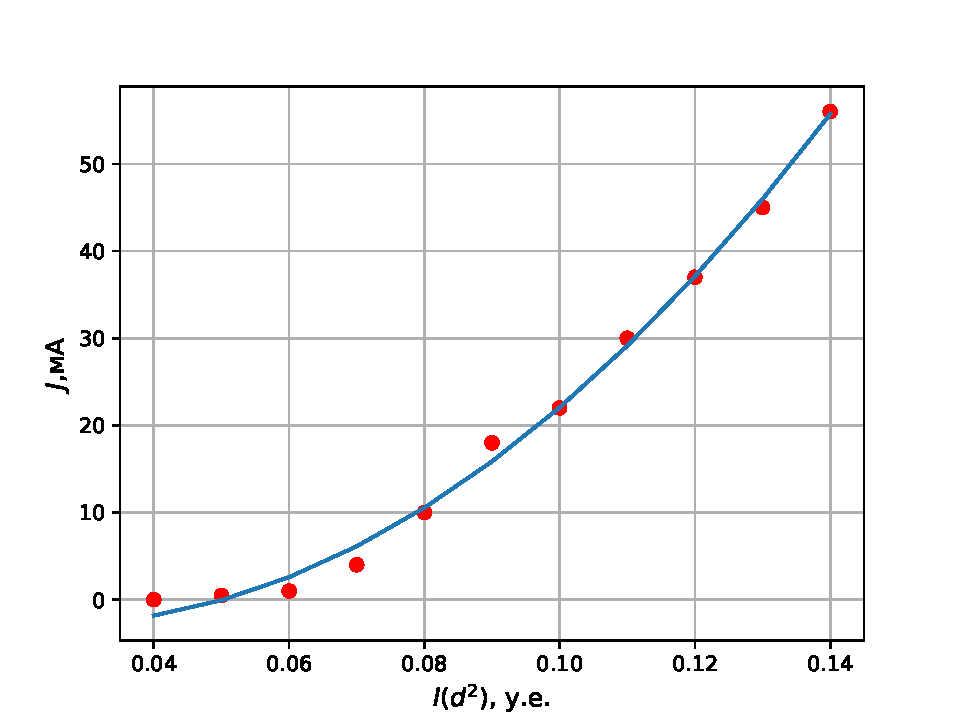
\includegraphics[scale=0.8]{scripts/2500}
% 	\caption{$2500^{\circ}$}
% 	\label{fig:5}
% \end{figure}

\subsection{Задание 2}
\begin{figure}[H]
	\centering
	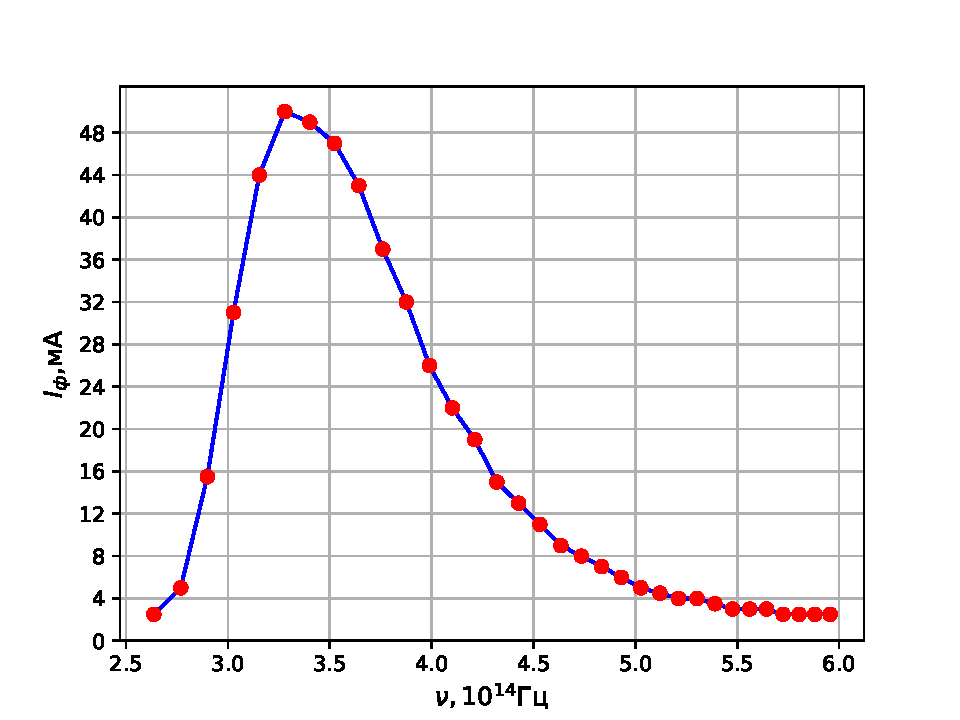
\includegraphics[scale=0.8]{scripts/n2}
	\caption{}
	\label{fig:6}
\end{figure}
Из рис. \ref{fig:6} мы можем определить красную границу фотоэффекта. Из него видно, что фототока нет при частоте, меньшей $\approx 2.9\cdot10^{14}$ Гц. 
\subsection{Задание 3}
\begin{figure}[H]
	\centering
	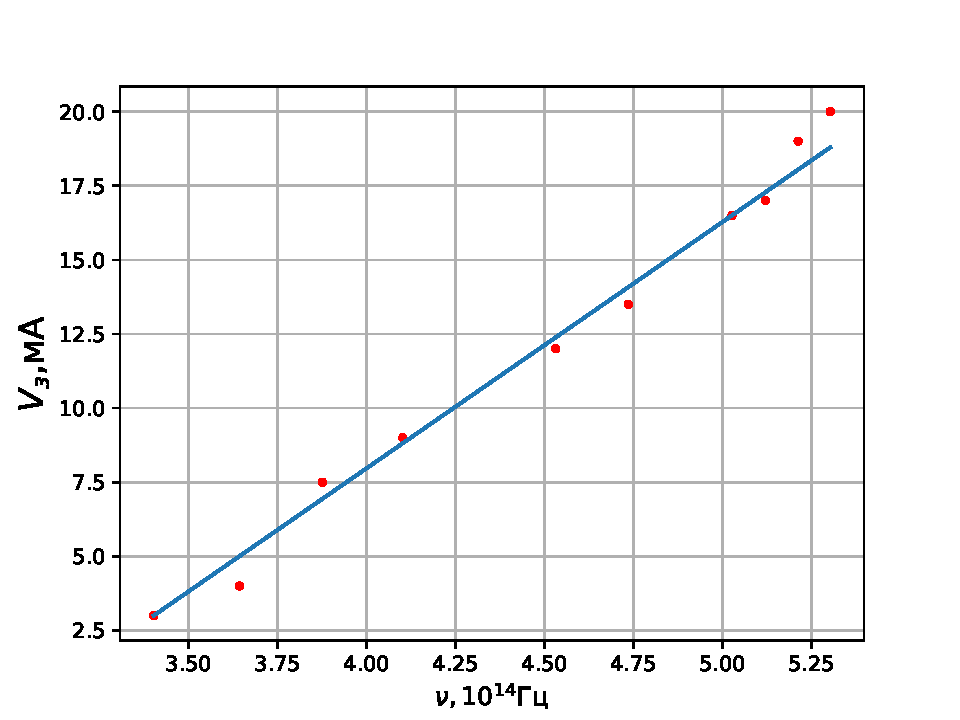
\includegraphics[scale=0.8]{scripts/n3}
	\caption{}
	\label{fig:7}
\end{figure}
Постоянную планка мы сможем найти из рис.\ref{fig:7}. Из \ref{eq:3} следует, что $\frac he$,равняется тангенсу угла наклона прямой. Возьмем из справочника заряд электрона $ e=1.60217733\cdot10^{-19}$ Кл и получаем, значение постоянной Планка $h=8.36\cdot10^{-34}\text{Дж}\cdot\text{с}$.

\end{document}
